% Exam Template for UMTYMP and Math Department courses
%
% Using Philip Hirschhorn's exam.cls: http://www-math.mit.edu/~psh/#ExamCls
%
% run pdflatex on a finished exam at least three times to do the grading table on front page.
%
%%%%%%%%%%%%%%%%%%%%%%%%%%%%%%%%%%%%%%%%%%%%%%%%%%%%%%%%%%%%%%%%%%%%%%%%%%%%%%%%%%%%%%%%%%%%%%

% These lines can probably stay unchanged, although you can remove the last
% two packages if you're not making pictures with tikz.
\documentclass[11pt]{exam}
\RequirePackage{amssymb, amsfonts, amsmath, latexsym, verbatim, xspace, setspace}
\RequirePackage{tikz, pgflibraryplotmarks}

% By default LaTeX uses large margins.  This doesn't work well on exams; problems
% end up in the "middle" of the page, reducing the amount of space for students
% to work on them.
\usepackage[margin=1in]{geometry}
\usepackage{enumerate}
\usepackage{amsthm}

\theoremstyle{definition}
\newtheorem{soln}{Solution}

% Here's where you edit the Class, Exam, Date, etc.
\newcommand{\class}{Math 150B Section 1}
\newcommand{\term}{Summer 2023}
\newcommand{\examnum}{Exam I}
\newcommand{\examdate}{July 16, 2023}
\newcommand{\timelimit}{1 Hour 10 Minutes}
\newcommand{\ol}[1]{\overline{#1}}

% For an exam, single spacing is most appropriate
\singlespacing
% \onehalfspacing
% \doublespacing

% For an exam, we generally want to turn off paragraph indentation
\parindent 0ex

\begin{document} 

% These commands set up the running header on the top of the exam pages
\pagestyle{head}
\firstpageheader{}{}{}
\runningheader{\class}{\examnum\ - Page \thepage\ of \numpages}{\examdate}
\runningheadrule

\begin{flushright}
\begin{tabular}{p{2.8in} r l}
\textbf{\class} & \textbf{Name (Print):} & \makebox[2in]{\hrulefill}\\
\textbf{\term} &&\\
\textbf{\examnum} & \textbf{Student ID:}&\makebox[2in]{\hrulefill}\\
\textbf{\examdate} &&\\
\textbf{Time Limit: \timelimit} % & Teaching Assistant & \makebox[2in]{\hrulefill}
\end{tabular}\\
\end{flushright}
\rule[1ex]{\textwidth}{.1pt}


This exam contains \numpages\ pages (including this cover page) and
\numquestions\ problems.  Check to see if any pages are missing.  Enter
all requested information on the top of this page, and put your initials
on the top of every page, in case the pages become separated.\\

You may \textit{not} use your books or notes on this exam.
You may use a single-sided, hand-written note sheet and a basic calculator.

You are required to show your work on each problem on this exam.  The following rules apply:\\

\begin{minipage}[t]{3.7in}
\vspace{0pt}
\begin{itemize}

%\item \textbf{If you use a ``fundamental theorem'' you must indicate this} and explain
%why the theorem may be applied.

\item \textbf{Organize your work}, in a reasonably neat and coherent way, in
the space provided. Work scattered all over the page without a clear ordering will 
receive very little credit.  

\item \textbf{Mysterious or unsupported answers will not receive full
credit}.  A correct answer, unsupported by calculations, explanation,
or algebraic work will receive no credit; an incorrect answer supported
by substantially correct calculations and explanations might still receive
partial credit.  This especially applies to limit calculations.

\item If you need more space, use the back of the pages; clearly indicate when you have done this.

\item \textbf{Box Your Answer} where appropriate, in order to clearly indicate what you consider the answer to the question to be.
\end{itemize}

Do not write in the table to the right.
\end{minipage}
\hfill
\begin{minipage}[t]{2.3in}
\vspace{0pt}
%\cellwidth{3em}
\gradetablestretch{2}
\vqword{Problem}
\addpoints % required here by exam.cls, even though questions haven't started yet.	
\gradetable[v]%[pages]  % Use [pages] to have grading table by page instead of question

\end{minipage}
\newpage % End of cover page

%%%%%%%%%%%%%%%%%%%%%%%%%%%%%%%%%%%%%%%%%%%%%%%%%%%%%%%%%%%%%%%%%%%%%%%%%%%%%%%%%%%%%
%
% See http://www-math.mit.edu/~psh/#ExamCls for full documentation, but the questions
% below give an idea of how to write questions [with parts] and have the points
% tracked automatically on the cover page.
%
%
%%%%%%%%%%%%%%%%%%%%%%%%%%%%%%%%%%%%%%%%%%%%%%%%%%%%%%%%%%%%%%%%%%%%%%%%%%%%%%%%%%%%%

\begin{questions}

\addpoints

\question[10]\mbox{}
Consider the area bounded by the curves $y=x$ and $x=y^3-3y$.

\begin{enumerate}[(a)]
\item  Draw a picture of the region bounded by the curves. Carefully label points of intersection between the curves.
\vspace{4in}
\item  Find the area of the region bounded by the curves.
\end{enumerate}



\newpage
\question[10]\mbox{} 

A grain silo lies in the shape of an inverted square pyramid of base length $4$ ft. and height $12$ ft. as featured below.
The silo is partially full of wheat, up to $8$ feet in height from the tip in the bottom.
Using the fact that wheat is $50$ lbs/ft$^3$, calculate the work required to pump all the wheat through the top of the tank.
Make sure to label your units!


\begin{center}
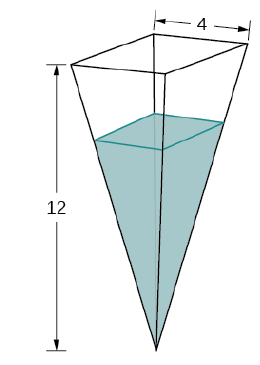
\includegraphics[height=2in]{grain.png}
\end{center}

\newpage
\question[10]\mbox{} 

Evaluate each of the following integrals.

\begin{enumerate}[(a)]
\item $\int e^{2x}\sin(3x)dx$
\vspace{4in}
\item $\int_0^{\pi/2} \sin^3(x)\cos^8(x)dx$
\end{enumerate}

\newpage
\question[10]\mbox{} 

Evaluate each of the following integrals.

\begin{enumerate}[(a)]
\item $\int \frac{3x^2}{\sqrt{4-x^2}}dx$
\vspace{4in}
\item $\int \frac{2x+3}{x^2(x+1)}dx$
\end{enumerate}

\newpage
\question[10]\mbox{} 

\begin{enumerate}[(a)]
\item Sketch a graph of the region bounded by $y=x^2$ and $y=2-x$.  Make sure to carefully label any points of intersection.
\vspace{2in}
\item Consider rotating the previous region around $x=2$ . Set up (but do not solve) an integral determining the volume using the Shell Method.
\vspace{3in}
\item Suppose instead that the region was rotated around the line $y=5$.  Set up (but do not solve) an integral determining the volume using the Disk/Washer Method.
\end{enumerate}

\end{questions}

\end{document}

